\chapter{مروری بر الگوریتم‌های هوش مصنوعی مورد بررسی}

در این بخش میخواهیم با انجام یک مرور برروی الگوریتم‌های مختلف هوش مصنوعی که برای پیشبینی کردن داده‌های سری زمانی
معمولا مورد استفاده قرار میگیرند آشنایی کلی با هریک از آن‌ها به‌دست بیاوریم.
بخش بزرگی از مسئولیت پیش‌بینی داده‌های سری زمانی برعهده ی یادگیری ماشین که خود یک بخش بزرگ از هوش مصنوعی میباشد هست.
از جمله الگوریتم‌های مهم در این بخش شبکه‌های عصبی مصنوعی، ماشین‌های بردار پشتیبان، میانگین متحرک خودهمبسته یکپارچه، سری زمانی فازی و استدلال مبتنی بر مورد هستند. 
در نهایت در پایان این بخش خلاصه ای از آنچه تابه حال در مورد این الگوریتم‌ها گفته شد خواهد امد.

\section{شبکه های عصبی مصنوعی}

شبکه‌های عصبی مصنوعی یک دسته از مدل‌های غیر‌خطی و غیر‌پارامتری هستند که برای تقریب عملکرد‌های غیر‌خطی و چند‌متغیره عمومی آموزش داده میشوند. 
این نوع شبکه‌ها سیستم‌های کاملا موازی هستند که از عناصر پردازشی به هم پیوسته به نام پرسپترون تشکیل شده‌اند.(پرسپترون یک شبیه سازی پایه ای از نورون مغز انسان هست)
یکی از مزایای اصلی شبکه‌های عصبی در مقایسه با مدل‌های دیگر عدم نیاز آن‌ها به داشتن فرضیات خاص میباشد.
در شکل \ref{fig:perceptron} از یک پرسپترون آمده است که نحوه ی کارکرد آن به طور کلی با تابع ریاضی زیر مدل میشود.

\begin{figure}[ht!]
    \begin{center}
        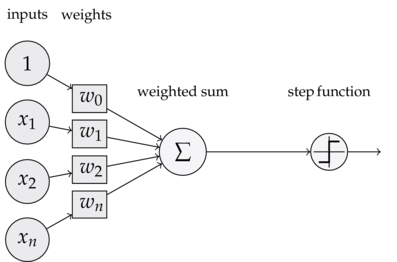
\includegraphics[width=7cm]{images/perceptron.png}
    \end{center}
    \caption[پرسپترون]{پرسپترون}
    \label{fig:perceptron}
    \end{figure}

\begin{equation}\label{eq:perceptron}
    output = f(\Sigma_{i = 1}^{n}(x_i*w_i) + w_0)
\end{equation}

در معادله ی \ref{eq:perceptron} ورودی‌های پرسپترون برابر با $x$ هستند و به تعداد ورودی‌های پرسپترون وزن‌های ‌$w_i$ در \ref{eq:perceptron} ورودی‌ها ضرب شده و حاصل جمع این عبارت به یک تابع فعال‌سازی در 
پرسپترون داده میشود. که در معادله ی بالا این تابع فعالسازی $f(x)$ فرض شده است.

شبکه ی عصبی مجموعه ای چندلایه از این پرسپترون ها میباشد که پرسپترون‌های هرلایه به تمام پرسپترون‌های لایه ی بعدی وصل شده و لایه‌ی ورودی ورودی‌های مسئله ی ما هستند و خروجی شبکه‌ی عصبی نیز خروجی خواسته شده‌ی ما هست.
در شکل \ref{fig:ann} یک شبکه ی عصبی نمونه آورده شده است.

\begin{figure}[ht!]
    \begin{center}
        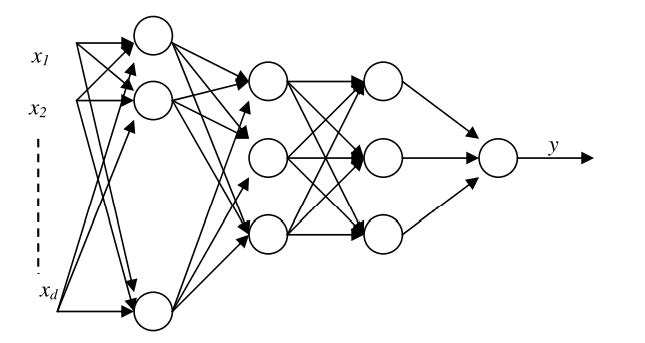
\includegraphics[width=12cm]{images/ANN.jpg}
    \end{center}
    \caption[شبکه‌ی عصبی مصنوعی]{شبکه‌ی عصبی مصنوعی}
    \label{fig:ann}
    \end{figure}

\section{ماشین بردار پشتیبان}

بر اساس اصل به حداقل رساندن خطر ساختاری از نظریه یادگیری آماری، ماشین بردار پشتیبان در ابتدا برای حل مسئله
شناسایی الگوی دو طبقه معرفی شد. ایده اصلی ساخت یک جداکننده است که در حالی که کوچکترین حاشیه را به حداکثر می
رساند )به عنوان مثال برای دستیابی به بزرگترین حاشیه از دو کلاس داده(، موارد مثبت و منفی را از هم جدا میکند. ماشین بردار
پشتیبان دو مزیت مهم دارد:
\begin{enumerate}
    \item انتخاب ویژگی اغلب مورد نیاز نیست، زیرا نسبت به بیشبرازش نسبتا قوی است و میتواند تا
    ابعاد بالا را مقیاسبندی کند.
    \item هیچ تلاشی در تنظیم پارامتر لازم نیست، زیرا نشان داده شده است که گزینه‌ی "پیش فرض" از
    لحاظ نظری، برای تنظیم بیشترین اثربخشی ارائه میشود
\end{enumerate} 

\noindent
از ماشین بردار پشتیبان برای حل دو نوع مسئله‌ی طبقه بندی و رگرسیون استفاده میشود. این روش در سال‌های گذشته عملکرد مناسبی در این دو مسئله داشته است.
این روش از جمله روش‌های نسبتا جدیدی است که در سال‌های اخیر کارایی خوبی نسبت به روش‌های قدیمی‌تر برای طبقه‌بندی نشان داده‌است. مبنای کاری دسته‌بندی کننده ماشین بردار پشتیبان دسته‌بندی خطی داده‌ها است و در تقسیم خطی داده‌ها سعی می‌کنیم خطی را انتخاب کنیم که حاشیه اطمینان بیشتری داشته باشد. قبل از تقسیم خطی برای اینکه ماشین بتواند داده‌های با پیچیدگی بالا را دسته‌بندی کند داده‌ها را به وسیله تابع $\phi$ به فضای با ابعاد خیلی بالاتر می‌بریم. برای اینکه بتوانیم مسئله ابعاد خیلی بالا را با استفاده از این روش‌ها حل کنیم از قضیه دوگانی لاگرانژ برای تبدیل مسئله مینیمم‌سازی مورد نظر به فرم دوگانی آن که در آن به جای تابع پیچیده $\phi$ که ما را به فضایی با ابعاد بالا می‌برد، تابع ساده‌تری به نام تابع هسته که ضرب برداری تابع $\phi$ است ظاهر می‌شود استفاده می‌کنیم. از توابع هسته مختلفی از جمله هسته‌های نمایی، چندجمله‌ای و سیگموید می‌توان استفاده نمود.
\\
به طور خلاصه برای ماشین بردار پشتیبان باید 
ماتریس الگو را آماده می‌کنیم. تابع کرنلی را برای استفاده انتخاب می‌کنیم. پارامتر تابع کرنل و مقدار $C$ را انتخاب می‌کنیم. برای محاسبه مقادیر$a_i$ الگوریتم آموزشی را با استفاده از حل‌کننده‌های $QP$ اجرا می‌کنیم. داده‌های جدید با استفاده از مقادیر$a_i$ و بردارهای پشتیبان می‌توانند دسته‌بندی شوند.
\\
هدف ماشین بردار پشتیبان به مانند شکل \ref{fig:svm} پیدا کردن دو ابرصفحه در حاشیه‌ی دو دسته از داده‌ها است که از یکدیگر بیشترین فاصله ی ممکن را داشته باشند.

\begin{figure}[ht!]
    \begin{center}
        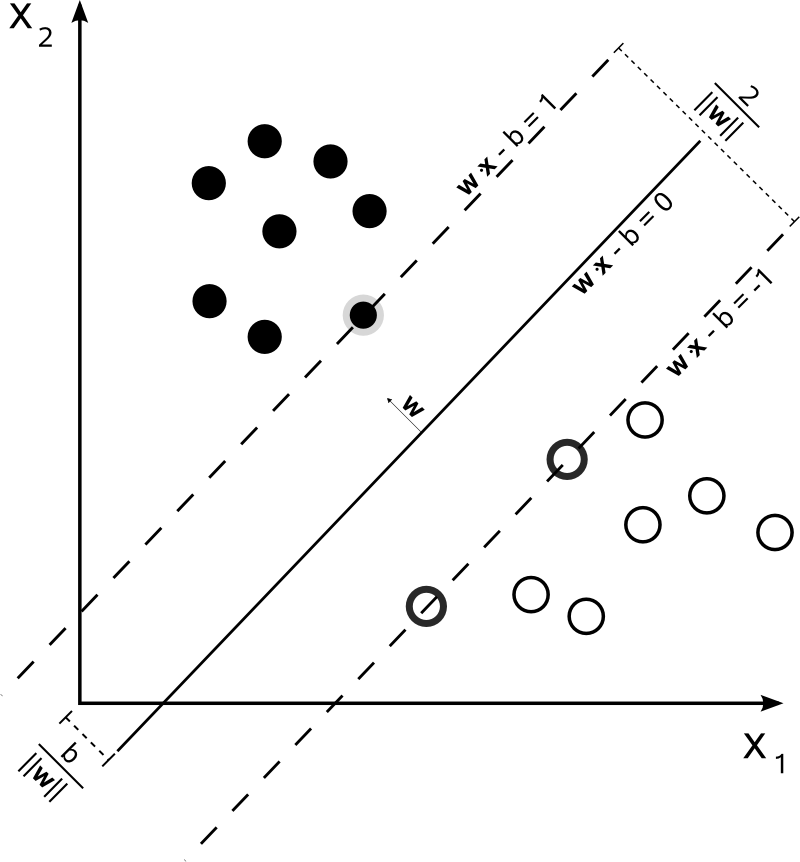
\includegraphics[width=12cm]{images/svm.png}
    \end{center}
    \caption[ماشین بردار پشتیبان]{ماشین بردار پشتیبان}
    \label{fig:svm}
    \end{figure}

\section[میانگین خودهمبسته یکپارچه]{میانگین متحرک خودهمبسته یکپارچه\protect\LTRfootnote{ARIMA}}
مدل‌های میانگین متحرک خودهمبسته یکپارچه اساسی‌ترین و عمومی‌ترین شکل تکنیک‌های پیش‌بینی سری‌های زمانی هستند. اینها بر اساس ایده تبدیل سری‌های زمانی به ثابت بودن توسط فرآیند تفاضل هستند. اگر خصوصیات آماری آن در طول زمان ثابت باشند، می‌توان سری زمانی را ثابت فرض کرد. بنابراین، معادله میانگین متحرک خودهمبسته  برای یک سری زمانی، یک معادله خطی است که ورودی آن شامل تاخیرهای متغیر وابسته به همراه تاخیرهای خطای پیش‌بینی است.
این مدل میتواند به صورت \ref{fig:ARIMA} توضیح داده بشود.

\begin{figure}[ht!]
    \begin{center}
        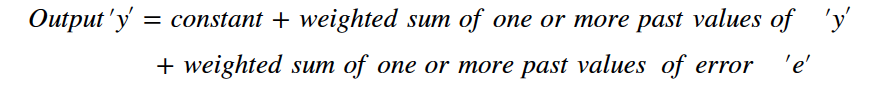
\includegraphics[width=12cm]{images/ARIMA.png}
    \end{center}
    \caption[میانگین متحرک خودهمبسته یکپارچه]{میانگین متحرک خودهمبسته یکپارچه}
    \label{fig:ARIMA}
    \end{figure}

\noindent
تأخیرهای عبارت خطا را نمی توان به عنوان متغیر مستقل در نظر گرفت زیرا آنها توابع خطی ضرایب نیستند. از این رو، ضرایب مدل‌های میانگین متحرک خودهمبسته یکپارچه 
با خطاهای تاخیری باید با تکنیک‌های دیگری مانند بهینه‌سازی غیرخطی محاسبه شوند. اصطلاحات تأخیر سری‌های زمانی ثابت به عنوان «خودرگرسیون» نامیده می شوند، 
در حالی که تأخیرهای عبارات خطای پیش‌بینی شده به عنوان «میانگین متحرک» نامیده می شوند. سری زمانی که برای ثابت کردن آن نیاز به تفکیک دارد،
    نسخه "یکپارچه" یک سری ثابت است.
    این مدل‌ها به صورت $ARIMA (p,d,q)$ نشان داده می‌شوند
، جایی که $p$ نشان‌دهنده ترتیب قسمت اتورگرسیو\LTRfootnote{autoregressive} $d$ درجه اولین تفاوت درگیر و $q$ نشان‌دهنده ترتیب قسمت میانگین متحرک است.
\noindent
بخش اتورگرسیو مدل با مرتبه $p$ مانند معادله\ref*{eq:autoregressive} نشان داده می‌شود.
\begin{equation}\label{eq:autoregressive}
    Y_t = c + \Phi_1 Y_{t-1} + \Phi_2 Y_{t-2} + \cdots + \Phi_p Y_{t-p} + e_t
\end{equation}

\noindent
 مدل میانگین متحرک $q$ نیز به صورت معادله \ref{eq:q} تعریف میشود:

\begin{equation}\label{eq:q}
    Y_t = c + \Theta_1 e_{t-1} + \Theta_2 e_{t-2} + \cdots + \Theta_p e_{t-p} + e_t
\end{equation}
\noindent
    جایی که $Y$ خروجی یک سری زمانی مانند داده های مصرف برق و $e_t$ سری خطا است. این مدل‌ها از یک روش رایج پیروی می‌کنند
\section{سری زمانی فازی}
سری‌های زمانی فازی مشاهدات سری زمانی با مقادیر زبانی هستند تا مقادیر عددی معمولی یا واضح مشاهدات.
 بنابراین، قوانین مرسوم تحلیل سری‌های زمانی را نمی توان برای مطالعه این موارد به کار برد. سانگ\LTRfootnote{Song} و چیسوم\LTRfootnote{Chissom} \cite{song1993fuzzy} این مفهوم را معرفی کردند و چندین تعریف رسمی برای سری‌های زمانی فازی ارائه کردند. 
 مطالعات بعدی بر تقسیم بندی جهان گفتمان و به دنبال آن ایجاد روابط فازی متمرکز شد. سپس مقادیر پیش‌بینی شده و برای به دست آوردن خروجی عددی غیرفازی می شوند. 
 لازم به ذکر است که انتخاب مناسب طول هر بازه فازی می تواند دقت پیش‌بینی را بسیار بهبود بخشد.
  برای مطالعات پیش‌بینی انرژی ساختمان، چالش در استخراج وزن‌های روابط منطق فازی، توابع عضویت و قوانین نهفته است.

\section[استدلال مبتنی بر مورد]{استدلال مبتنی بر مورد\protect\LTRfootnote{Case-based reasoning}}
استدلال مبتنی بر مورد مبتنی بر یادآوری اطلاعات از یک پرونده قبلی برای حل یک پرونده جدید است. مخالف با ایده استخراج قواعد از مشاهدات که می تواند در یک مجموعه عمومی اعمال شود است.
 بلکه این فرآیند متکی بر موارد مشابهی است 
 که در گذشته به آن پرداخته شده است و نه چندان متدولوژی حل آنها.
  منبع دانش اولیه در استدلال مبتنی بر مورد حافظه ای از موارد ذخیره شده است که قسمت های قبلی خاص را ضبط می کند\cite{leake1996cbr}. 
 فرمول اولیه این مفهوم برگرفته از مطالعه نقش یادآوری در استدلال انسان است\cite{schank1983dynamic}. 
 استدلال مبتنی بر مورد در کاربرد خود در پیش‌بینی مصرف انرژی ساختمان، مواردی را در نظر می‌گیرد که دارای انواع مشابهی از متغیرهای ورودی هستند
  و سعی می‌کند بر اساس سناریوهای مشابه قبلی مدل‌سازی کند.

\section[مدل‌های ترکیبی]{مدل‌های ترکیبی‌\protect\LTRfootnote{Hybrid Models}}
مدل های ترکیبی ترکیبی از دو یا چند تکنیک یادگیری ماشینی هستند. این مدل‌ها قوی‌تر هستند، 
زیرا اغلب مزایای تکنیک‌های فردی درگیر را تحسین می‌کنند و دقت پیش‌بینی را بهبود می‌بخشند.
متد‌های بسیار متنوعی برای مدل‌های ترکیبی پیاده‌سازی و تست شده‌اند. از میان انبوهی از این مدل‌ها می‌توانیم به چند مورد زیر اشاره بکنیم:
\begin{itemize}
    \item شبکه‌های عصبی مصنوعی و الگوریتم‌های تکاملی
    \item ماشین بردار پشتیبان و میانگین متحرک خودهمبسته یکپارچه
    \item شبکه عصبی فازی در حال تکامل وزنی
    \item شبکه‌ی عصبی مصنوعی و میانگین متحرک خودهمبسته یکپارچه
    \item ...
\end{itemize}
\noindent
لازم به ذکر است که توضیحات مربوط به پیچیدگی‌های ساختن مدل‌های ترکیبی، طبقه‌بندی آن‌ها و موارد استفاده هریک آز آن‌ها متاسفانه در این بخش پرداخته نشده‌اند و تنها به ذکر چند مدل گسترده استفاده شده از آن‌ها بسنده کرده‌ایم.
\section{خلاصه}

با توجه به توضیحات داده شده ی بالا هر یک از این الگوریتم‌ها مزایا و معایب خودشان را در کار عملی پیش‌بینی داده‌های سری زمانی نشان خواهند داد. 
 در مسیر پیش‌بینی داده‌های زمانی مصرف انرژی ساختمان‌ها از الگوریتم‌های مختلفی همچون 
 ماشین بردار پشتیبان، شبکه‌های عصبی مصنوعی، میانگین متحرک خودهمبسته یکپارچه، سری زمانی فازی، استدلال مبتنی بر مورد و مدل‌های ترکیبی استفاده شده است.
 به طور کلی مدل‌های متنوع دیگری نیز در این مسئله وجود دارند که قادر به ارائه‌ی نتایج دقیق به متخصصین هستند. نکته‌ی بسیار مهم در این الگوریتم‌ها این است که اغلب آن‌ها به تنهایی و بدون داشتن مجموعه‌ی داده‌های آموزشی که کیفیت مناسبی را دارند
 کارایی چندان مناسبی نخواهند داشت. لازم به ذکر است که الگوریتم‌های هوش‌مصنوعی نیازمند منابع محاسباتی گسترده‌ای هستند که خود این امر یک محدودیت برای آن‌ها به حساب می‌آید.
 در صورتی که هریک از این موارد برای این الگوریتم‌ها رعایت نشوند یعنی داده‌های زیاد و با کیفیت و همچنین ارائه‌ی سیستم‌های قدرتمند برای انجام محاسبات به نتیجه ی مطلوب و دلخواه نخواهیم رسید.